\chapter{مدل دامنه}
مدل دامنه، یک فرایند مفهوم‌سازی برای کمک به تیم توسعه جهت فهم دامنه‌ی کاربرد است که دارای پنج گام مختلف می‌باشد.
\begin{itemize}
	\item
	جمع‌آوری اطلاعات دامنه‌‌ی کاربردی
	\item
	طوفان فکری
	\item
	دسته‌بندی نتایج طوفان فکری
	\item
	به تصویر کشیدن مدل دامنه
	\item
	مرور و بازرسی مدل دامنه
\end{itemize}

\section{جمع‌آوری اطلاعات دامنه کاربردی}
مقصود اصلی از مدل‌سازی دامنه، فهم مفاهیم دامنه و چگونگی ارتباط آن‌ها با یکدیگر است، در این مرحله اعضای تیم باید مستندات یا توضیحات موجود در مورد کسب‌و‌کار را بدست آورد.
\section{طوفان فکری}
پس از جمع‌آوری اطلاعات،‌اعضای تیم در قالب ۲ جلسه به شناسایی مفاهیم مهم دامنه پرداختند، که محصول نهایی این گام که با توجه به قوانین زیر بدست آمده، فهرستی از عبارت‌های شناخته شده است.
\begin{enumerate}
	\item
	اسم‌‌ها یا عبارات اسمی
	\item
	عبارت‌های
	\lr{x} از \lr{y}
	یا
	\lr{y x}
	\item
	افعال متعدی
	\item
	صفات، قید‌‌ها و اقلام شمارشی
	\item
	ارقام و اعداد و کمیت‌ها
	\item
	عبارت‌ها مالکیت
	\item
	اجزای سازنده، عبارت‌های
	\underline{تشکیل شده از} و
	\underline{بخشی از}
	\item
	عبارت‌های مربوط به دربرداشتن
	\item
	عبارت‌های
	\lr{X}
	یک
	\lr{Y}
	یا مفاهیم خاص کردن / تعمیم دادن است.
\end{enumerate}

\section{دسته‌بندی نتایج طوفان فکری}
در این مرحله اعضای گروه به دسته‌بندی مفاهیم دامنه پرداختند.

\section{فهرست مفاهیم مهم دامنه}
این فهرست در جدول \ref{table:domain} نوشته شده است.

\begin{longtable}{|c|c|c|}
	\hline		لیست طوفان فکری &		نتیجه‌ی دسته‌بندی &		قانون \\
	\hline
	\hline		حساب کاربری &
	\myc &
	\onealef \\
	\hline		نام &
	\mya &
	\oneh \\
	\hline		نام خانوادگی &
	\mya &
	\oneh \\
	\hline		کد ملی &
	\mya &
	\oneh \\
	\hline		ایمیل &
	\mya &
	\oneh \\
	\hline		تاریخ تولد &
	\mya &
	\oneh \\
	\hline		شماره تلفن &
	\mya &
	\oneh \\
	\hline		کد اتباع &
	\mya &
	\oneh \\
	\hline		تحصلیات &
	\myc &
	\onej \\
	\hline		رزومه &
	\mya &
	\oneh \\
	\hline		محل سکونت &
	\mya &
	\oneh \\
	\hline		نام کاربری &
	\mya &
	\oneh \\
	\hline		رمز عبور &
	\mya &
	\oneh \\
	\hline		علایق &
	\myc &
	\onej \\
	\hline		دسته‌بندی&
	\myc &
	\onej \\
	\hline		وضعیت تاهل &
	\mya &
	\oneh \\
	\hline		احراز هویت کردن &
	\asus &
	3 \\
	\hline		خرید اکانت پرمیوم &
	\asus &
	3 \\
	\hline		ساختن حساب‌کاربری &
	\asus &
	3 \\
	\hline		مشاهده‌ی حساب‌کاربری &
	\asus &
	3 \\
	\hline		ویرایش حساب‌‌کاربری &
	\asus &
	3 \\
	\hline		دیدن آگهی‌های شغلی &
	\asus &
	3 \\
	\hline		تغییر رمز عبور &
	\asus &
	3 \\
	\hline		بازیابی رمزعبور فراموش شده &
	\asus &
	3 \\
	\hline		کارجو &
	\myc &
	\oned \\
	\hline
	نشاندار کردن آگهی		&
	\asjs &
	3 \\
	\hline
	دخیره کردن آگهی &
	\asjs &
	3 \\
	\hline
	دادن درخواست شغلی &
	\asje &
	3 \\
	\hline
	ساخت رزومه &
	\asjs &
	3 \\
	\hline
	آپلود رزومه &
	\asjs &
	3 \\
	\hline
	ارسال رزومه &
	\asje &
	3 \\
	\hline
	جستجو کردن در آگهی‌ها &
	\asus &
	3 \\
	\hline
	فیلتر کردن آگهی‌ها &
	\asus &
	3 \\
	\hline
	کارفرما &
	\myc &
	\oned \\
	\hline
	مشاهده‌ی کارجویان پیشنهادی &
	\ases &
	3 \\
	\hline
	مشاهده‌ی پروفایل کارجویان &
	\asus &
	3 \\
	\hline
	ارسال پیام دعوت به همکاری &
	\asej &
	3 \\
	\hline
	مشاهده‌ی رزومه‌ی کارجویان &
	\asus &
	3 \\
	\hline
	پاسخ دادن به درخواست‌ها &
	\aser &
	3 \\
	\hline
	قبول کردن درخواست &
	\aser &
	3 \\
	\hline
	رد کردن درخواست &
	\aser &
	3 \\
	\hline
	ثبت آگهی‌ شغلی &
	\ases &
	3 \\
	\hline
	بارگزاری پروانه‌ی کسب &
	\ases &
	3 \\
	\hline
	ثبت شرکت & 
	\ases & 
	3 \\
	\hline
	نام شرکت & 
	\mya & 
	\oneh \\
	\hline
	شماره‌ی ثبت شرکت & 
	\mya & 
	\oneh \\
	\hline
	شماره‌ی تماس شرکت & 
	\mya & 
	\oneh \\
	\hline
	آدرس شرکت & 
	\mya & 
	\oneh \\
	\hline
	ایمیل شرکت & 
	\mya & 
	\oneh \\
	\hline
	لیست آگهی‌های شرکت & 
	\mya & 
	\oneh \\
	\hline
	زمینه‌ی کاری شرکت & 
	\mya & 
	\oneh \\
	\hline
	عکس شرکت & 
	\mya & 
	\oneh \\
	\hline
	رتبه‌ی شرکت & 
	\mya & 
	\oneh \\
	\hline
	علامت تجاری شرکت & 
	\mya & 
	\oneh \\
	\hline
	هویت سنجی مکانی & 
	\asse & 
	3 \\
	\hline
	تطبیق آگهی با رزومه & 
	\assj & 
	3 \\
	\hline
	بازیابی اطلاعات کاربران & 
	\assu & 
	3 \\
	\hline
	۲۰ ثانیه & 
	\myv & 
	\fiveb \\
	\hline
	چت کردن & 
	\asje & 
	3 \\
	\hline
	۱۰۰۰۰ کاربر & 
	\myv & 
	\fiveb \\
	\hline
	\caption{مفاهیم مهم دامنه}\label{table:domain}
\end{longtable}

\section{به تصویر کشیدن مدل دامنه}
مدل دامنه در تصویر \ref{pic:dm} آورده شده است.
\begin{figure}[h]
	\begin{center}
		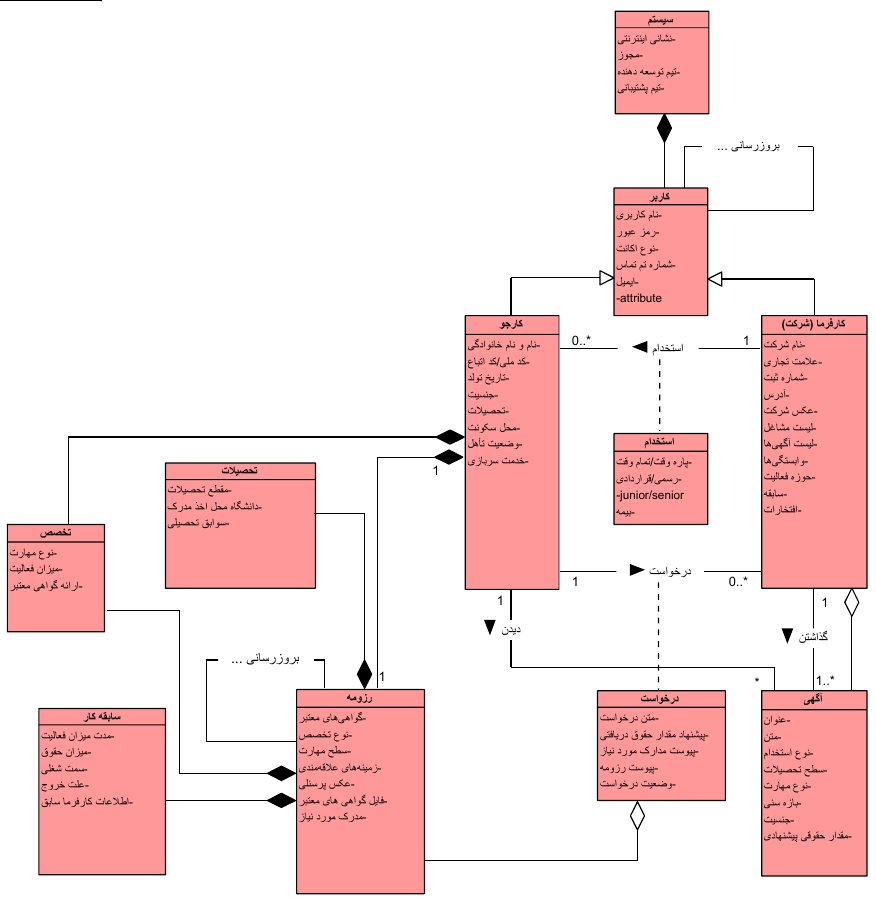
\includegraphics[width=0.7\textwidth, height=0.5\textheight, angle=90]{./images/dm}
	\end{center}
\caption{مدل دامنه}
\label{pic:dm}
\end{figure}
\section{مرور مدل دامنه}
پس از انجام همه‌ی مراحل، اعضای تیم بار دیگر به بررسی مدل دامنه می‌پردازند و در صورت وجود هرگونه اشکال آن را اصلاح می‌کنند.

\section{رعایت اصول چابکی}
کلیه مراحل مدل‌سازی دامنه با درنظر گرفتن اصول چابکی انجام شده و تیم توسعه با درنظر گرفتن کاربرد سامانه‌ی \textit{کارتاپ} و در جهت شناسایی بهتر نیازمندی‌ها سعی کرده است که با مشتری تعامل لازم را داشته باشد تا جلوی بروز هرگونه ابهام را بگیرد.

همچنین برای جلوگیری از پیچیده‌ شدن مدل دامنه در بخش طوفان فکری همه‌ی کلاس‌ها به یک باره ذکر نشده‌اند و مراحل به صورت گام‌به‌گام انجام شده چون فرایند مدل‌سازی یک فرایند تکراری‌ست و باید بازگشت‌پذیر باشد.